\section*{Introduction}
Avant de présenter les travaux antérieurs relatifs à la gestion numérique 
des activités administratives municipales, il convient d'introduire un 
certain nombre de notions fondamentales qui seront mobilisées tout au long 
de ce mémoire. Cette section a pour objectif de clarifier les concepts clés 
et de poser les bases terminologiques de notre étude.

% ============================================================
\section{Généralités}
% ============================================================

\subsection{Application web}
Une application web est un logiciel accessible via un navigateur internet 
qui permet de gérer des données et des services en ligne, sans nécessiter 
d'installation préalable sur le poste de l'utilisateur.

\subsection{Travaux dirigés}
Les Travaux dirigés (TD) désignent des séances d'encadrement scolaire 
organisées en dehors des cours réguliers, destinées à préparer les 
candidats aux examens officiels. Dans le cadre de ce projet, ils sont 
financés et administrés par les services de la commune de Cotonou.

\subsection{Gestion administrative}
La gestion administrative désigne l'ensemble des processus visant à 
organiser, planifier, suivre et contrôler les activités et ressources 
d'une organisation. Elle englobe la gestion des données, des flux 
financiers et la production de rapports décisionnels.

\subsection{Collectivité locale}
Une collectivité locale désigne une entité administrative territoriale 
dotée d'une personnalité juridique propre et d'une autonomie de gestion. 
La commune de Cotonou, dans le cadre de ce projet, représente la 
collectivité locale commanditaire de la solution développée.

\subsection{Tableau de bord}
Un tableau de bord est un outil de pilotage qui centralise et affiche en 
temps réel les indicateurs clés d'une activité. Il permet aux décideurs 
de suivre l'état des opérations et d'orienter leurs actions de manière 
rapide et éclairée.

\subsection{Paiement électronique}
Le paiement électronique désigne tout mode de règlement financier effectué 
par voie numérique, qu'il s'agisse de virement bancaire en ligne ou de 
paiement via une plateforme sécurisée.

% ============================================================
\section{Présentation des solutions existantes}
% ============================================================

Dans le domaine de la gestion administrative des activités municipales, 
plusieurs approches ont été adoptées afin d'organiser le suivi des travaux 
dirigés. Nous présentons ici trois solutions représentatives, en mettant en 
lumière leurs fonctionnalités principales, leurs avantages, ainsi que leurs 
limites dans le cadre d'une adaptation au contexte béninois.

% ----------------------------
\subsection{Gestion manuelle sur registres papier}
% ----------------------------

La figure~\ref{fig:registre} présente un extrait du registre traditionnel 
utilisé par les services municipaux pour consigner les informations 
relatives aux travaux dirigés.

\begin{figure}[H]
    \centering
    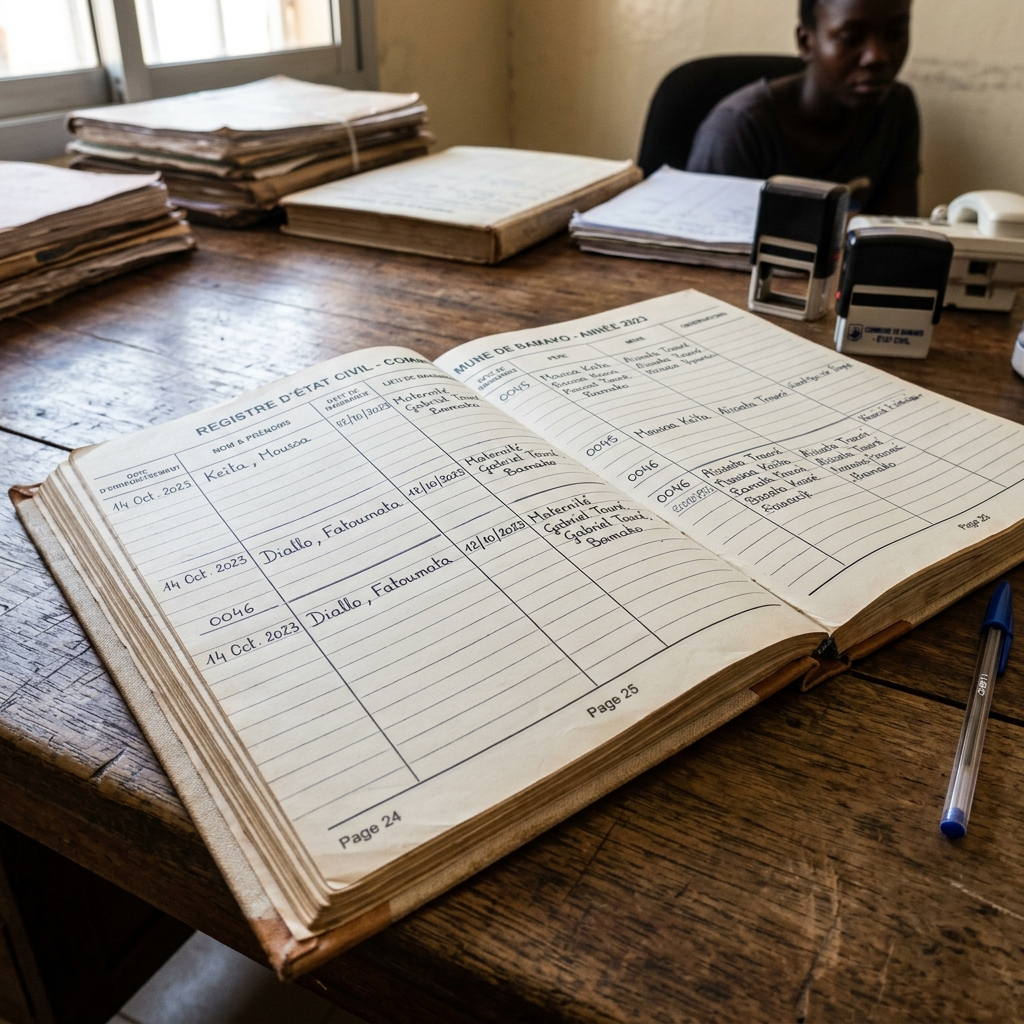
\includegraphics[width=0.7\textwidth]{images/registre_papier.png}
    \caption{Exemple de registre manuel (Source : terrain)}
    \label{fig:registre}
\end{figure}

Cette méthode, bien que simple, présente de nombreuses contraintes :

\begin{itemize}
    \item \textbf{Risque de perte :} Risque de perte, de déchirure ou de dégradation du support, 
    entraînant la disparition définitive des informations.
    \item \textbf{Lenteur de recherche :} Difficulté à retrouver rapidement les données, rendant le suivi 
    des paiements et des sessions lent et peu fiable.
    \item \textbf{Manque de traçabilité :} Absence totale de traçabilité financière et d'automatisation 
    des traitements.
\end{itemize}

% ----------------------------
\subsection{Gestion sur tableurs (Microsoft Excel / Google Sheets)}
% ----------------------------

Microsoft Excel et Google Sheets sont des outils bureautiques largement 
utilisés dans les administrations locales pour gérer des données 
tabulaires. La figure~\ref{fig:excel} illustre un exemple d'utilisation 
dans un contexte administratif.

\begin{figure}[H]
    \centering
    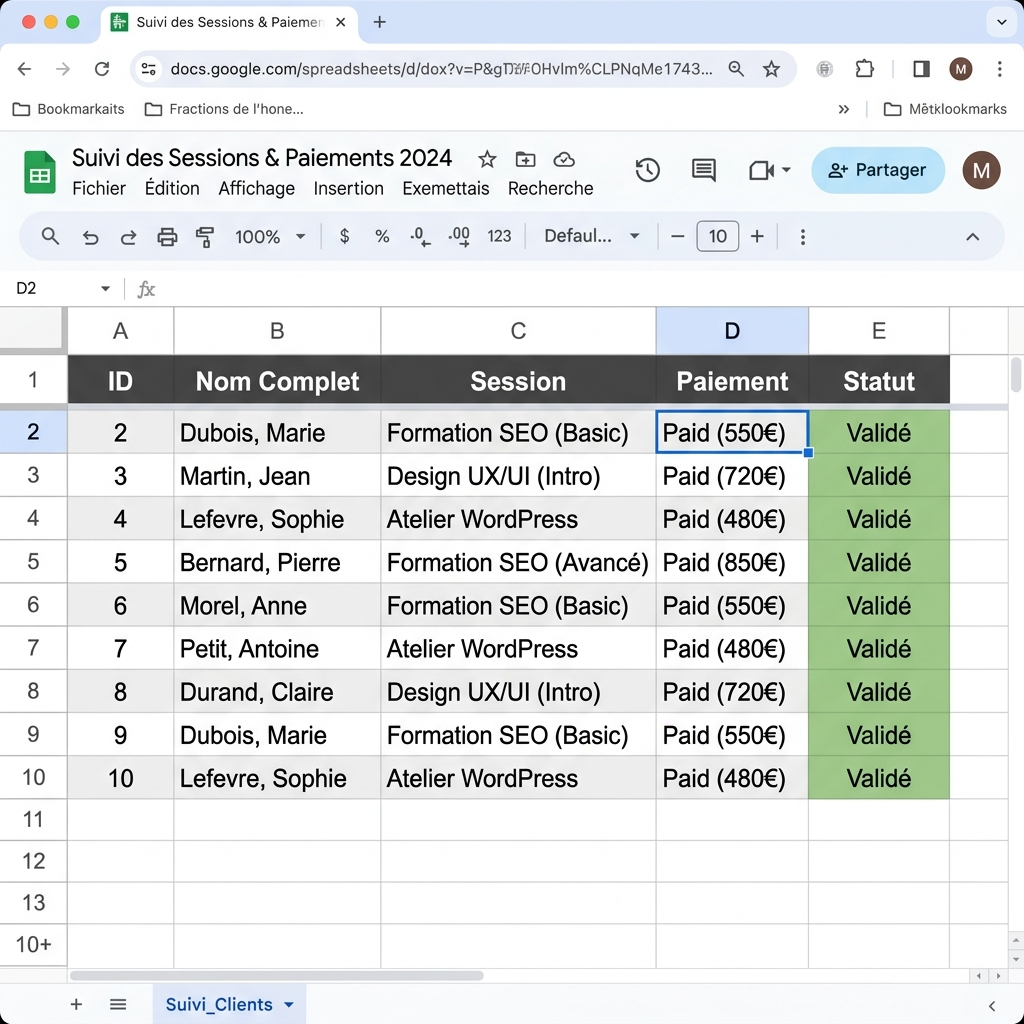
\includegraphics[width=0.8\textwidth]{images/excel_sheets.png}
    \caption{Interface Excel / Google Sheets (Source : \cite{microsoft})}
    \label{fig:excel}
\end{figure}

\textbf{Elle présente les avantages suivants :}
\begin{itemize}
    \item Facilité de prise en main et accessibilité ;
    \item Calculs automatisés et mise en forme des données ;
    \item Partage de fichiers possible via Google Drive.
\end{itemize}

Cependant, cette solution présente des limites significatives :
\begin{itemize}
    \item Absence de sécurisation des accès et des données ;
    \item Pas de tableau de bord dynamique ni de reporting automatisé ;
    \item Risque élevé d'erreurs humaines lors des saisies ;
    \item Inadaptée à une gestion multi-utilisateurs en temps réel.
\end{itemize}

% ----------------------------
\subsection{Logiciel de gestion généraliste --- Odoo}
% ----------------------------

Odoo est un ERP open source offrant des modules de gestion administrative, 
financière et comptable. La figure~\ref{fig:odoo} illustre son interface 
principale.

\begin{figure}[H]
    \centering
    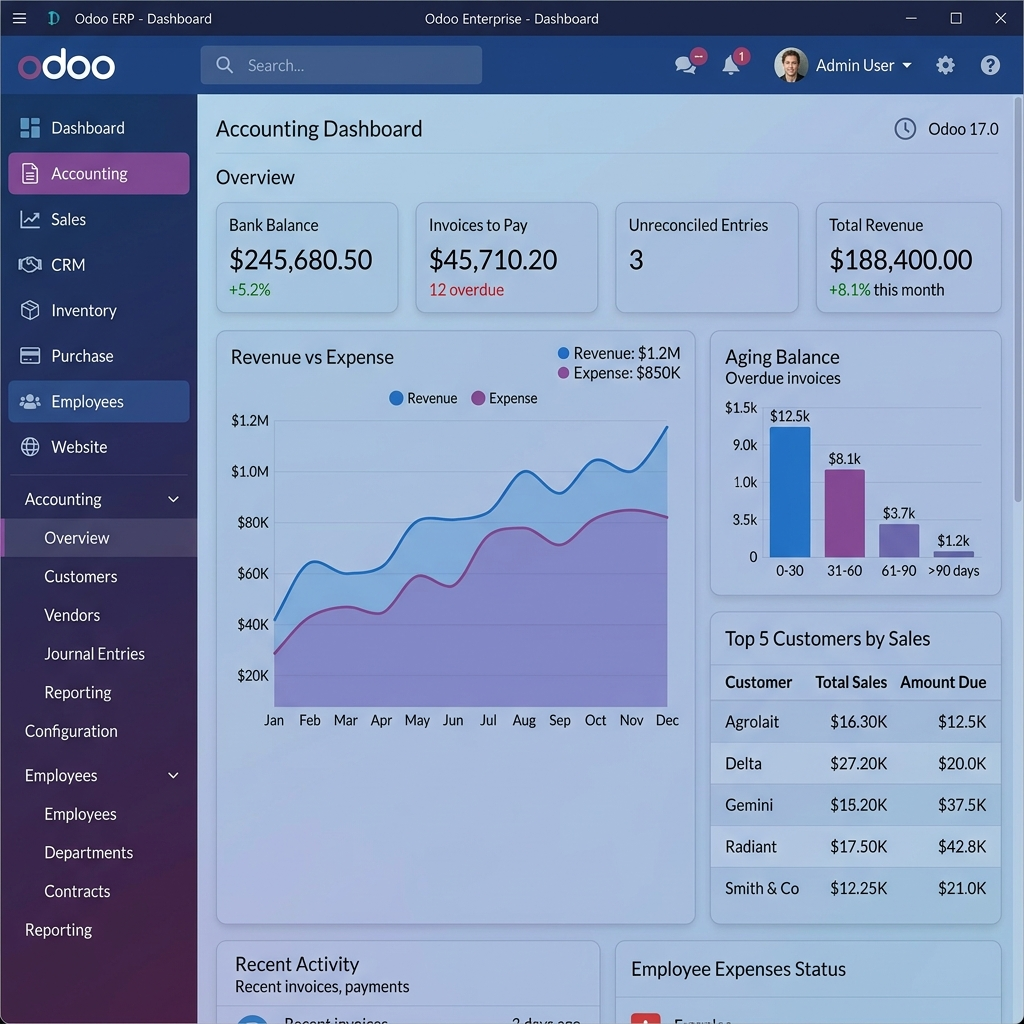
\includegraphics[width=0.8\textwidth]{images/odoo_interface.png}
    \caption{Interface Odoo (Source : \cite{odoo})}
    \label{fig:odoo}
\end{figure}

\textbf{Elle présente les avantages suivants :}
\begin{itemize}
    \item Gestion centralisée des données et des flux financiers ;
    \item Tableau de bord interactif et reporting avancé ;
    \item Système d'authentification et gestion des droits utilisateurs ;
    \item Automatisation des paiements et des notifications.
\end{itemize}

Ses limites dans notre contexte sont néanmoins notables :
\begin{itemize}
    \item Coût de déploiement et de maintenance élevé ;
    \item Complexité d'utilisation nécessitant une formation approfondie ;
    \item Non adapté à la gestion spécifique des travaux dirigés municipaux ;
    \item Dépendance à une infrastructure technique solide.
\end{itemize}

% ----------------------------
\subsection{Tableau comparatif des solutions étudiées}
% ----------------------------

Le tableau~\ref{tab:comparaison} ci-dessous présente une comparaison 
synthétique des trois solutions étudiées.

\begin{table}[H]
\centering
\caption{Tableau comparatif des solutions existantes}
\label{tab:comparaison}
\renewcommand{\arraystretch}{1.5}
\setlength{\tabcolsep}{10pt}
\begin{tabular}{|l|c|c|c|}
\hline
\rowcolor{gray!20} \textbf{Critères} & \textbf{Registre papier} & \textbf{Excel/Sheets} & \textbf{Odoo} \\
\hline
Centralisation des données     & \ding{55} & Partielle & \ding{51} \\
Tableau de bord interactif     & \ding{55} & \ding{55}  & \ding{51} \\
Automatisation des paiements   & \ding{55} & \ding{55}  & \ding{51} \\
Génération de rapports         & \ding{55} & Partielle & \ding{51} \\
Sécurité des accès             & \ding{55} & \ding{55}  & \ding{51} \\
Adaptation au contexte local   & \ding{51} & \ding{51}  & \ding{55} \\
Coût accessible                & \ding{51} & \ding{51}  & \ding{55} \\
Facilité d'utilisation         & \ding{51} & \ding{51}  & \ding{55} \\
\hline
\end{tabular}
\end{table}

% ----------------------------
\subsection{Analyse critique des solutions existantes}
% ----------------------------

Les solutions présentées révèlent plusieurs insuffisances lorsqu'elles 
sont confrontées aux réalités des services municipaux béninois. La gestion 
manuelle sur papier ne garantit ni la fiabilité ni la traçabilité des 
opérations. Les tableurs, bien qu'accessibles, restent non sécurisés et 
inadaptés à une gestion multi-utilisateurs structurée. Enfin, des solutions 
comme Odoo, malgré leurs capacités techniques avancées, s'avèrent trop 
coûteuses, trop complexes et non spécifiquement conçues pour la gestion 
des travaux dirigés dans une commune béninoise. Aucune de ces solutions ne 
répond donc de manière complète, ciblée et accessible aux besoins identifiés.

% ============================================================
\section{Intérêt de la solution par rapport aux existantes}
% ============================================================

\begin{itemize}
    \item \textbf{Interface intuitive et adaptée au contexte local :} 
    l'application est pensée pour les agents administratifs municipaux, 
    sans nécessiter de formation technique approfondie.

    \item \textbf{Solution ciblée et spécialisée :} contrairement aux 
    outils généralistes, notre application est conçue spécifiquement pour 
    la gestion des travaux dirigés, avec des fonctionnalités directement 
    alignées sur les besoins opérationnels de la commune.

    \item \textbf{Tableau de bord analytique personnalisé :} un module 
    statistique offre une visibilité en temps réel sur les indicateurs 
    clés : sessions, paiements, états financiers.

    \item \textbf{Automatisation des paiements :} la plateforme intègre 
    l'envoi de fichiers de paiement aux banques et le traitement des 
    paiements électroniques, fonctionnalité absente des solutions 
    existantes accessibles localement.

    \item \textbf{Accessibilité multi-appareils :} la solution est 
    responsive et accessible depuis tout appareil connecté sans 
    installation préalable.

    \item \textbf{Évolutivité :} l'architecture technique retenue permet 
    d'étendre les fonctionnalités selon les besoins futurs de la commune.
\end{itemize}

% ============================================================
\section*{Conclusion}
% ============================================================

Ce chapitre a permis de poser les bases conceptuelles de notre étude et 
d'analyser les solutions existantes dans le domaine de la gestion 
administrative. Il ressort clairement qu'aucune solution disponible ne 
répond de façon complète, ciblée et économiquement accessible aux besoins 
de la commune de Cotonou en matière de gestion des travaux dirigés. Ces 
constats justifient pleinement le développement d'une application web 
dédiée, dont l'analyse, la conception et la réalisation font l'objet des 
chapitres suivants.
